\documentclass[12pt]{report} 

\usepackage{fancyhdr}
\usepackage[french]{babel}
\usepackage[utf8]{inputenc}
\usepackage{graphicx}
\usepackage{float}

\usepackage{geometry}
 \geometry{
 a4paper,
 total={170mm,257mm},
 left=20mm,
 top=20mm,
 }

 % \textsubscript defined equivalent to \textsuperscript in latex.ltx
\DeclareRobustCommand*\textsubscript[1]{%
  \@textsubscript{\selectfont#1}}
\def\@textsubscript#1{%
  {\m@th\ensuremath{_{\mbox{\fontsize\sf@size\z@#1}}}}}

% Title Page
\title{Mathématiques - Recherche opérationnelle \\
TP noté Python \\
\textbf{Voyageur de commerce}}
\author{Benjamin LE GALLO \\
Steven PELLIET \\
C2}

\begin{document}
\pagenumbering{arabic}
\maketitle
\thispagestyle{empty}

\tableofcontents

\chapter{Introduction}
 
Le voyageur de commerce est un \textbf{problème d'optimisation} qui, étant donné une liste de villes, 
et des distances entre toutes les paires de villes, \textbf{détermine un plus court chemin qui visite chaque ville 
une et une seule fois et qui termine dans la ville de départ}. \\

C'est un problème algorithmique célèbre, qui a généré beaucoup de recherches et qui est souvent utilisé comme 
introduction à l'algorithmique ou à la théorie de la complexité. Il présente de nombreuses applications que ce soit 
en planification et en logistique, ou bien dans des domaines plus éloignés comme la génétique 
(en remplaçant les villes par des gènes et la distance par la similarité). \\

Résoudre un problème d'optimisation, c'est trouver une valeur des paramètres d'un problème qui donne une solution 
meilleure que les autres. Une façon de trouver les meilleurs paramètres consiste à essayer toutes les valeurs possibles.
Lorsque le nombre de paramètres possibles est grand cela peut se révéler impraticable.\\

Une technique mise au point dans les années 1960 est inspirée de la sélection naturelle: il s'agit 
des \textbf{algorithmes génétiques}. \\

\begin{figure}[!htb]
\minipage{0.32\textwidth}
  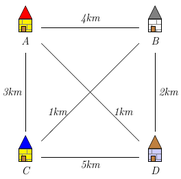
\includegraphics[width=\linewidth]{img/pb1}
  \caption{Instance du problème}\label{fig:pb1}
\endminipage\hfill
\minipage{0.32\textwidth}
  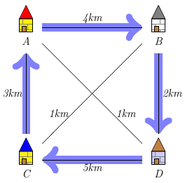
\includegraphics[width=\linewidth]{img/pb2}
  \caption{Possible solution du problème}\label{fig:pb2}
\endminipage\hfill
\minipage{0.32\textwidth}%
  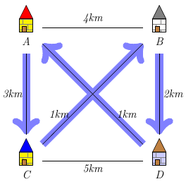
\includegraphics[width=\linewidth]{img/pb3}
  \caption{Solution optimale du problème}\label{fig:pb3}
\endminipage
\end{figure}

\cleardoublepage
\chapter{Algorithmes génétiques}

La \textbf{sélection naturelle} permet de sélectionner les individus les mieux adaptés à l'environnement (Darwin). Cette sélection
par \textbf{reproduction}: les individus sélectionnés se reproduisent en mélangeant leurs gènes, et ce sont les individus les mieux 
adaptés qui se reproduisent le plus. Ils transmettent leurs gènes (qui sont supposés être le mieux adaptés) à leur descendance.
Ainsi, sur une population nombreuse et un grand nombre de générations, les gènes les mieux adaptés seront de plus en plus
représentés dans la population. D'autres processus d'évolution du matériel génétique existent dans la nature: les \textbf{mutations}. \\

Les algorithmiques génétiques sont \textbf{une manière de mimer le processus de sélection naturelle} décrit plus haut. On suppose que
l'on connaît une fonction-objectif qui à \textbf{chaque individu associe un nombre qui évalue sa performance} (par convention: plus 
la valeur est basse, meilleure est la performance). On cherche un individu qui a une valeur de la fonction-objectif minimale. \\
Chaque individu \textbf{dépend d'un certain nombre de paramètres} que l'on peut coder dans une chaîne (par exemple binaire) de longueur
\textit{l}. Générer tous les individus possibles est hors de portée car on se place dans un cas où le nombre total
de paramètres possibles est très grand.

\begin{figure}[H]
\centering
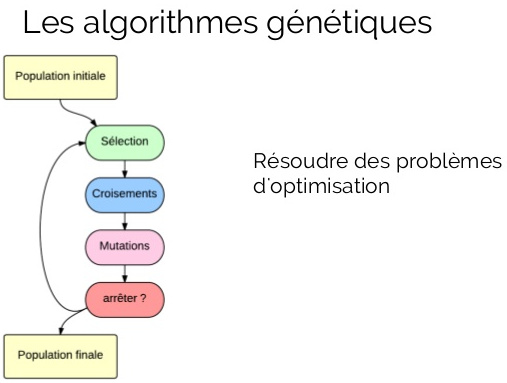
\includegraphics[scale=0.74]{img/algo-genetic}
\caption{Illustration de l'algorithme génétique}
\end{figure}

\section{Principe des algorithmes génétiques}

Un individu est \textbf{une solution du problème}. Une population représente \textbf{tous les individus, toutes les solutions}.


\section{Sélection}

La méthode par sélection permet \textbf{d'éliminer des individus, les solutions les moins adaptées}.

\section{Croisement}

La méthode par croisement consiste à croiser deux individus (parents), qui produisent \textbf{deux nouvelles solutions} (enfants).

\section{Mutation}

La méthode par mutation consiste \textbf{à modifier aléatoirement un individu, une solution}.

\section{Adaptation}

La méthode d'adaption consiste \textbf{à évaluer un individu, une solution par rapport au problème à résoudre}.

\cleardoublepage
\chapter{Fonctionnement (Python)}

\section{Étapes}

\subsection{Initialisation}
Voici les étapes d'initialisation nécessaire avant de commencer les itérations qui permet de ne garder que les meilleurs solutions.\\
\begin{itemize}
\item \textbf{Création de la map}, elle représente la distance entre chaque ville
\item \textbf{Générer des solutions (population)}, créer un certain nombre de solutions (définis par l'utilisateur), ces solutions représentent l'ordre des villes à parcourir pour obtenir une solution optimale
\end{itemize}

\subsection{Générations (itérations)}
Les générations consistent à "filtrer" la population (solutions) avec des méthodes spécifiques inspirées de la génétique (sélection, croisement, mutation). La population finale contiendra les ``meilleures solutions''. Cependant les solutions seront approximative car il ne faut pas oublier qu'il s'agit d'un problème d'optimatisation. L'objectif est de se rapprocher de la solution optimale !\\
\begin{itemize}
 \item \textbf{Sélection par élitisme}, elle consiste à retourner une population (m) plus performante
\item \textbf{Sélection par roulette}, elle consiste à choisir au hasard deux solutions et ne conservera
que la meilleure des deux pour ensuite retourner une population (m) plus performante
\item \textbf{Croisement}, permet de créer de nouvelles solutions se rapprochant des meilleures solutions actuelles, pour obtenir une population (2m). 
\item \textbf{Mutation}, elle échange deux villes dans une solution, elle permet elle aussi de se rapprocher de la solution optimale
\end{itemize}

\subsection{Résultat}
\begin{itemize}
 \item \textbf{Sélection de la solution optimale}, il s'agit de ne garder que la meilleure solution, la solution optimale
 \item \textbf{Ordre des villes}, il s'agit d'afficher l'ordre des villes à parcourir avec la distance optimale
 \item \textbf{Calcul de la distance parcourue}, à partir de la map et de la meilleure solution, elle retourne la distance à parcourir
\end{itemize}

\section{Éxecution}
Voici un exemple de résolution du problème du voyageur de commerce par un utilisateur.\\

\begin{figure}[H]
\centering
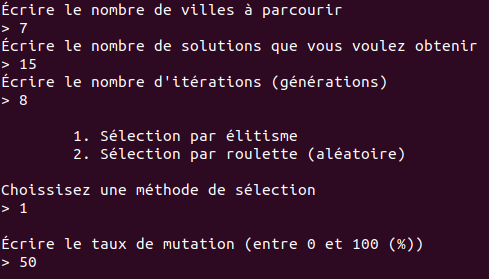
\includegraphics[scale=0.85]{img/initialization}
\caption{Initialisation des variables}
\end{figure}

\begin{figure}[H]
\centering
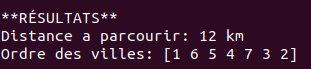
\includegraphics[scale=1]{img/results}
\caption{Résolution du problème du voyageur de commerce}
\end{figure}

\chapter{Annexe}

\section{Questions}

\textbf{Question 1:} Combien y a t-il d'individus possibles qui sont codés par une chaîne binaire de longueur \textit{l} = 100 ?

\begin{flushleft}
    \textbf{Réponse:}\\
    3 individus possibles
    \begin{itemize}
    \item 001
    \item 010
    \item 100
    \end{itemize}
\end{flushleft}

\textbf{Question 2:} Combien y a t-il de permutations des entiers \textit{1..n} ? Est-il envisageable de toutes les énumérer lorsque \textit{n} = 10 ? \textit{n} = 30 ?

\begin{flushleft}
    \textbf{Réponse:}\\
    Il y a \textbf{n!} permutations possibles des entiers. Il n'est évidemment pas envisageable de tous les énumérer quand n est grand. Pour \textit{n} = 10, il existe \textbf{3 628 800} permutations possibles et pour \textit{n} = 30, \textbf{2.652 528 60\textsuperscript{32}}.
\end{flushleft}
 
\end{document}   
